\documentclass[a4paper]{article}
\usepackage[utf8x]{inputenc}
\usepackage[T1]{fontenc}
\usepackage[MeX]{polski}
\usepackage{amssymb}
\usepackage{graphicx}
\usepackage{subcaption}
\usepackage{fancyhdr}
\usepackage{lastpage}
\usepackage{xcolor}

\pagestyle{fancy}
\fancyhf{}
\cfoot{ \thepage \hspace{1pt} / \pageref{LastPage}}
\lhead{Sprawozdanie ko\'ncowe}
\rhead{\texttt{GameOfLife}}


\begin{document}

\begin{titlepage}
	\begin{center}
		\vspace*{5cm}

	        \Huge
        	\textbf{Sprawozdanie ko\'ncowe}

        	\vspace{1cm}
	        \Huge
        	\texttt{GameOfLife}: Gra w \.zycie Johna Conwaya

    		\vspace{1.5cm}

	        \large
		Aleksandra Michalska, Natalia Olszewska

        	\vfill

	        \vspace{3cm}

		\large 05.04.2021
	\end{center}
\end{titlepage}

\tableofcontents
\newpage


\part{Informacje og\'olne}

\section{O dokumencie}
\quad Dokument jest podsumowaniem projektu \textit{\texttt{GameOfLife}: Gra w \.zycie Johna Conwaya}. 
Koresponduje z dokumentami \textit{"Specyfikacja funkcjonalna automatu kom\'orkowego"} oraz \textit{"Specyfikacja implementacyjna automatu kom\'orkowego"}.

\section{O programie}
\quad Program jest implementacj\k{a} "Gry w \.Zycie" Johna Conwaya. Zosta\l{} rozszerzony o dodatkowe zasady obliczania s\k{a}siedztwa oraz rodzaje \'swiat\'ow. 

\section{\'Srodowisko implementacyjne i funkcjonalne}
\quad Program zosta\l{} zaimplementowany w j\k{e}zyku programowania \textbf{C} w systemie operacyjnym \textbf{Linux} (dystrybucja Ubuntu). 
W celu kontroli wersji zosta\l{}y u\.zyte \textbf{GitHub} (utworzenie wst\k{e}pnej wersji projektu) oraz \textbf{Projektor EE}, b\k{e}d\k{a}cy systemem kontroli wersji Politechniki Warszawskiej (utoworzenie ostatecznej wersji projektu). 
\\
\\
Pozosta\l{}ymi u\.zytymi narz\k{e}dziami by\l{}y:
\begin{itemize}
	\item \textbf{ImageMagick} - otwieranie zapisanych przez u\.zytkownika obraz\'ow
	\item \textbf{Valgrind} - przeprowadzenie test\'ow wyciek\'ow pami\k{e}ci
	\item \textbf{Vim} - podstawowa edycja kodu
	\item \textbf{Evince} - otwieranie dokumentacji plik\'ow o rozszerzeniu \textbf{pdf}
	\item \textbf{\LaTeX{}} - tworzenie dokumentacji
	\item \textbf{Make} - utworzenie pliku \textbf{Makefile} i wywo\l{}anie programu
\end{itemize}


\newpage
\part{Funkcjonalno\'sci programu}

\section{Uruchomienie}
\quad Program mo\.zna uruchomi\'c korzystaj\k{a}c z samodzielnie dobranych parametr\'ow podstawowych i dodatkowych (patrz punkty 4.1.1 oraz 4.1.2) 
lub z gotowych polece\'n zaimplementowanych w \textbf{Makefile} (\textbf{\texttt{make run\_sbs}}, \textbf{\texttt{make run\_fast}}, 
\textbf{\texttt{make no\_save}}, \textbf{\texttt{make after\_change}}).

\subsection{Parametry wej\'sciowe}
\subsubsection{Parametry podstawowe}
\quad Z powodu kwestii implementacyjnych, spos\'ob u\.zycia nast\k{e}puj\k{a}cych parametr\'ow uleg\l{} zmianie: 
\begin{itemize}
	\item \textbf{\texttt{ -in filein.txt }} zosta\l{} zast\k{a}piony \textbf{\texttt{ -{}-in filein.txt}}
	\item \textbf{\texttt{ -out fileout.txt }} zosta\l{} zast\k{a}piony \textbf{\texttt{ -{}-out fileout.txt}}
	\item \textbf{\texttt{ -how(Ms || Mf || Ns || Nf) }} zosta\l{} zast\k{a}piony \textbf{\texttt{ -{}-how(Ms || Mf || Ns || Nf || Ps || Pf)}}, przy czym:
		\begin{itemize}
			\item \textbf{\texttt{s}} "sphere world" pozostaje bez zmian (patrz \textit{"Specyfikacja funkcjonalna automatu kom\'orkowego"})
			\item \textbf{\texttt{f}} "flat world" zosta\l{} zmodfikowany. 
				W tym \'swiecie, dla kom\'orek: 
				\\- na rogach, uznawanych jest \textbf{3} s\k{a}siad\'ow (patrz \textit{Rysunek \ref{fig:n3}}),
				\\- na obrze\.zach, uznawanych jest \textbf{5} s\k{a}siad\'ow (patrz \textit{Rysunek \ref{fig:n5}}), 
				\\- w \'srodku, uznawanych jest \textbf{8} s\k{a}siad\'ow (patrz Rysunek \textit{\ref{fig:n8}}). 
				\\ \\ Zasady umierania i powracania do \.zycia, w trybach podstawowych, pozostaj\k{a} takie same.  
		\end{itemize} 
		Nowe rodzaje ustalania s\k{a}siedztwa tj. \textbf{\texttt{Pf}} oraz \textbf{\texttt{Ps}}, zosat\l{}y opisane w punkcie 4.3.3.
		

\begin{figure}[h!]
        \centering
        \begin{subfigure}[b]{0.2\linewidth}
                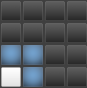
\includegraphics[width=\linewidth]{neighbour3}
                \caption{Kom\'orka w rogu}
                \label{fig:n3}
        \end{subfigure}
        \hspace{1.5cm}
        \begin{subfigure}[b]{0.2\linewidth}
                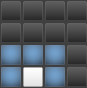
\includegraphics[width=\linewidth]{neighbour5}
                \caption{Kom\'orka na brzegu}
                \label{fig:n5}
        \end{subfigure}
        \hspace{1.5cm}
        \begin{subfigure}[b]{0.2\linewidth}
                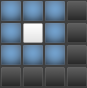
\includegraphics[width=\linewidth]{neighbour8}
                \caption{Kom\'orka w \'srodku}
                \label{fig:n8}
        \end{subfigure}
        \label{fig:sasiedzi}
        \caption{Rozmieszczenie s\k{a}siad\'ow dla poszczeg\'olnych kom\'orek w p\l{}askim \'swiecie}
\end{figure}

	\item \textbf{\texttt{ -s(o2 || f2) }} zosta\l{} wycofany z parametr\'ow obowi\k{a}zkowych (patrz punkt 4.1.2)
\end{itemize}

Spos\'ob u\.zycia pozosta\l{}ych parametr\'ow pozostaje niezmieniony (patrz \textit{"Specyfikacja funkcjonalna automatu kom\'orkowego"}).

Przyk\l{}adowe poprawne parametry wej\'sciowe:


\begin{center}
	\textbf{\texttt{./game -{}-in plikin.txt -{}-out plikout.txt -n 20 -m sbs -{}-how Ps}}
\end{center}


\subsubsection{Parametry dodatkowe}
\quad U\.zytkownik ma mo\.zliwo\'s\'c skorzystania z dodatkowych, nieobowi\k{a}zkowych parametr\'ow:
\begin{enumerate}
\item Przy kompilacji programu:
	\begin{itemize}
		\item \textbf{\texttt{ -DIN='"path\_to\_dir\_input"' }} zmiana \'scie\.zki do katalogu, z kt\'orego pobierane b\k{e}d\k{a} pliki wej\'sciowe 
			\\(domy\'slny katalog: \textbf{\texttt{'"Generacje\_Wej\'sciowe"'}})
		\item \textbf{\texttt{ -DOUT='"path\_to\_dir\_output"' }} zmiana \'scie\.zki do katalogu, w kt\'orym zapisywane b\k{e}d\k{a} pliki wyj\'sciowe
			\\(domy\'slny katalog: \textbf{\texttt{'"Generacje\_Wyj\'sciowe"'}})
		\item \textbf{\texttt{ -DSIZE=10 }} zmiana rozmiaru boku jednej kom\'orki (w pikselach) w generowanym obrazie (domy\'slny rozmiar: 40)
		\item \textbf{\texttt{ -DHOW\_FAST=200000 }} zmiana odst\k{e}pu czasu (w mikrosekundach) pomi\k{e}dzy wy\'swietlaniem kolejnych generacji w trybie \textbf{\texttt{FAST}} (domy\'slny czas: 210000)
	\end{itemize}
\item Przy uruchamianiu programu:
	\begin{itemize}
		\item \textbf{\texttt{ -s (o2 || f2)}} spos\'ob u\.zycia pozostaje niezmieniony (patrz \textit{"Specyfikacja funkcjonalna automatu kom\'orkowego"})
	\end{itemize}
\end{enumerate}




\subsection{Obs\l{}uga podstawowa}
\quad U\.zytkownik uruchamia program przy pomocy gotowych polece\'n zaimplementowanych w \textbf{Makefile}. Przyk\l{}adowo, komenda:
\begin{center}
	\textbf{\texttt{make run\_fast}}
\end{center}
oznacza polecenie:
\begin{center}
	\textbf{\texttt{./game -{}-in starship.txt -{}-out wunik.txt -s f5 -n 20 -{}-how Ms -m fast}}
\end{center}

\quad U\.zytkownik ma tak\.ze mo\.zliwo\'s\'c korzystania z samodzielnie dobranych parametr\'ow (patrz punkt 4.1). 


\subsection{Obs\l{}uga szczeg\'o\l{}owa}
\subsubsection{Tryb \texttt{SBS}}
\quad Tryb \texttt{SBS} umo\.zliwia przechodzenie do kolejnych generacji po wci\'sni\k{e}ciu dowolnego klawisza poza klawiszem \textbf{\textit{e}}. 
Je\.zeli u\.zytkownik poda wi\k{e}cej ni\.z 1 klawisz, program pobierze tylko ostatni lub klawisz \textbf{\textit{e}}, je\.zeli pojawi\l{} si\k{e} w\'sr\'od wybranych. 
\\
Przyk\l{}adowo, podanie liter \textbf{\textit{aaaaaab}} oznacza dla programu to samo, co podanie klawisza \textbf{\textit{b}}, 
natomiast podanie liter \textbf{\textit{aaaeaab}} oznacza tyle co naci\'sni\k{e}cie klawisza \textbf{\textit{e}}. 


Zosta\l{} tak\.ze zmieniony spos\'ob prze\'scia z trybu \texttt{SBS} do trybu \texttt{FAST}. 
Zamiast wybrania klawisza \textbf{\textit{f}} u\.zytkownik powinien wybra\'c klawisz \textbf{\textit{e}}.  

\subsubsection{Tryb \texttt{FAST}}
\quad W tym trybie u\.zytkownik nie wchodzi w interakcj\k{e} z programem, kolejne generacje wy\'swietlane s\k{a} automatycznie. 
U\.zytkownik nie ma mo\.zliwo\'sci zmiany tego trybu na inny ani przerwania pracy programu (poza wymuszeniem, kt\'ore powoduje przerwanie pracy Makefile'a).

\subsubsection{Rodzaj ustalania s\k{a}siedztwa \texttt{PERSONAL}}
\quad W programie zosta\l{} zaimplementowany nowy spos\'ob ustalania s\k{a}siedztwa na podstawie preferencji u\.zytkownika. Aby z niego skorzysta\'c, nale\.zy przy wywo\l{}aniu u\.zy\'c jednego z poni\.zszych parametr\'ow:
\begin{itemize}
	\item \textbf{\texttt{ -{}-how Ps }} czyli w\l{}asny spos\'ob ustalania s\k{a}siedztwa, \'swiat dzia\l{}aj\k{a}cy jak sfera
	\item \textbf{\texttt{ -{}-how Pf }} czyli w\l{}asne spos\'ob ustalania s\k{a}siedztwa, \'swiat dzia\l{}aj\k{a}cy jak p\l{}aska plansza
\end{itemize}

\quad W przypadku wybrania tego trybu, zostaje wy\'swietlony interface, w kt\'orym u\.zytkownik wybiera jak chce ustala\'c s\k{a}siedztwo:


\begin{figure}[h!]
	\centering
	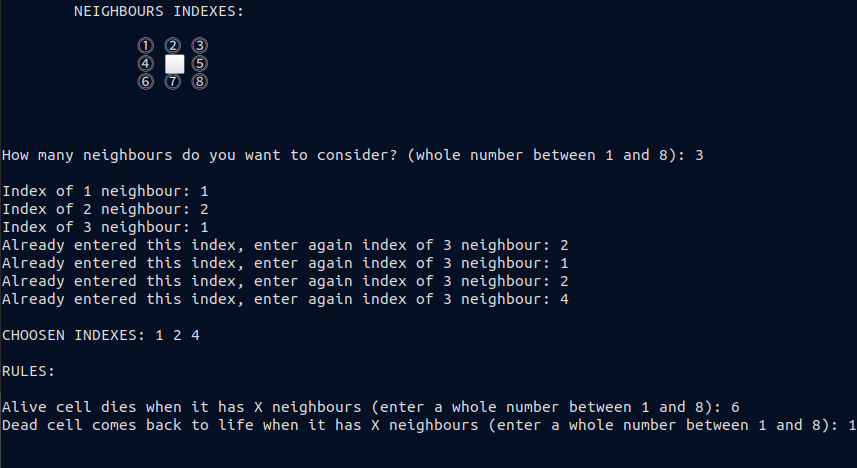
\includegraphics[width=\linewidth]{personalmode}
	\caption{Ustawianie w\l{}asnych zasad s\k{a}siedztwa}
        \label{fig:interface}
\end{figure}


\section{Dodatkowe funkcje}
\quad W celu u\l{}atwienia korzystania z programu u\.zytkownik ma mo\.zliwo\'s\'c skorzystania z komend pomocniczych:
\begin{itemize}
	\item \textbf{\texttt{ make remove\_out }} umo\.zliwia usuni\k{e}cie wszystkich plik\'ow wyj\'sciowych z katalogu z generacjami wyj\'sciowymi
	\item \textbf{\texttt{ make remove\_image }} umo\.zliwia usuni\k{e}cie wszystkich obraz\'ow z katalogu \textbf{\texttt{Obrazy}}
\end{itemize}


\section{Wyniki dzia\l{}ania programu}


\subsection{Wy\'swietlanie generacji w terminalu}
\quad Kolejne generacje wy\'swietlne s\k{a} w terminalu (patrz \textit{Rysunek \ref{fig:fast}} i \textit{Rysunek \ref{fig:sbs1}}). 
Wy\'swietlana jest tak\.ze informacja o numerze obecnej generacji oraz liczbie \.zywych kom\'orek.

\begin{figure}[h!]
        \centering
        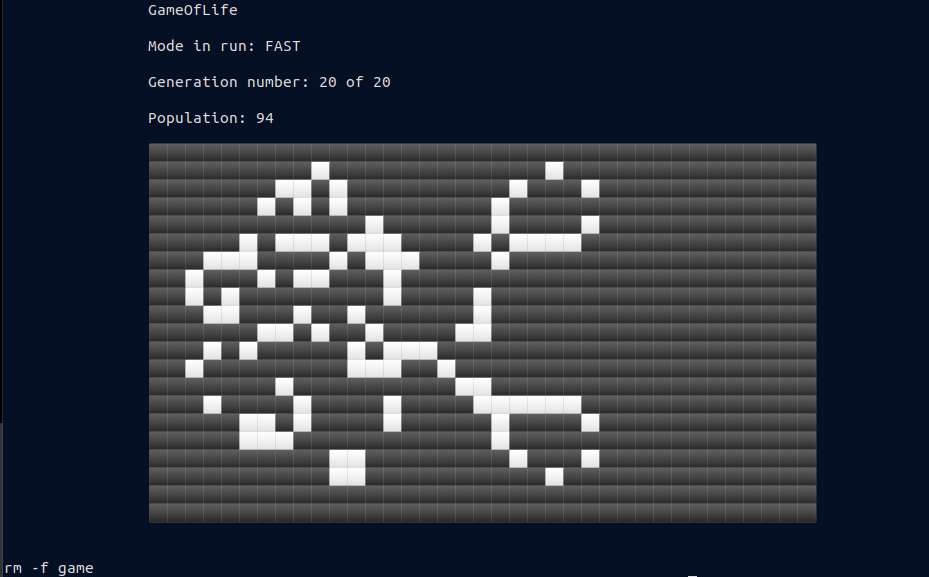
\includegraphics[scale=0.28]{FAST}
	\caption{Interface trybu \texttt{FAST}}
        \label{fig:fast}
\end{figure}

\begin{figure}[h!]
        \centering
	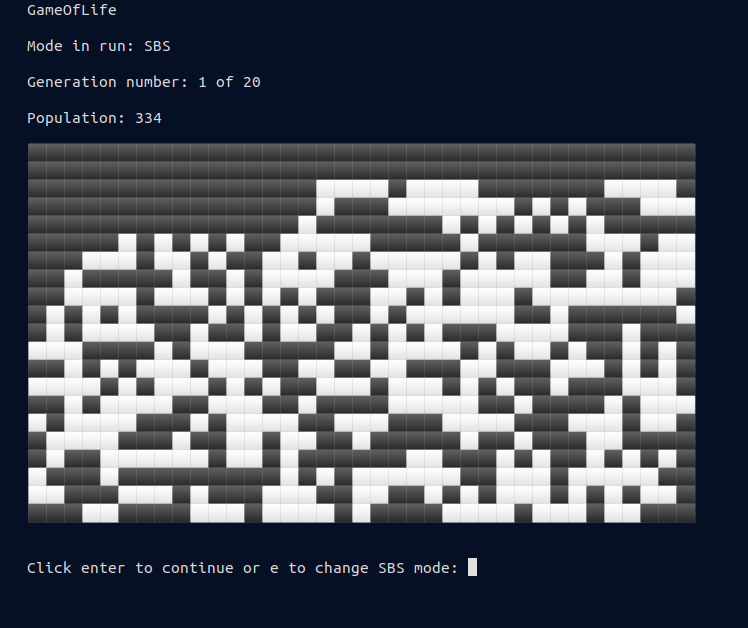
\includegraphics[scale=0.28]{sbs1}
	\caption{Interface trybu \texttt{SBS}}
        \label{fig:sbs1}
\end{figure}

\newpage

\subsection{Zapis plik\'ow graficznych}
\quad Wybrane przez u\.zytkownika generacje mo\.zna wy\'swietli\'c przy u\.zyciu programu takiego jak ImageMagick (patrz \textit{Rysunek \ref{fig:imagemagik}}).

\begin{figure}[h!]
        \centering
        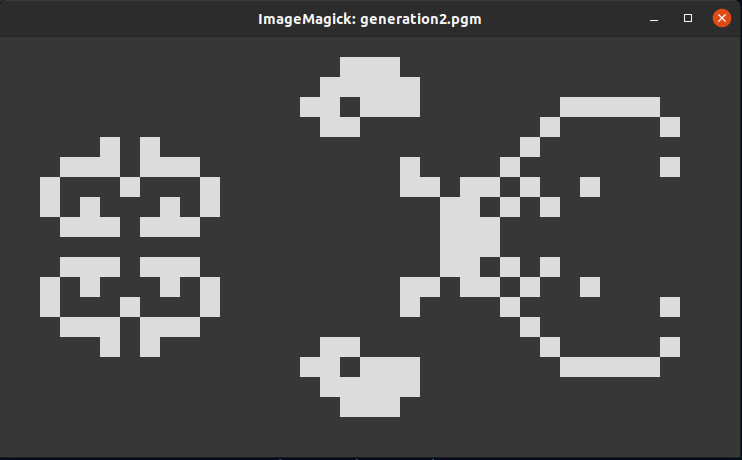
\includegraphics[scale=0.4]{imagemagik}
	\caption{Wy\'swietlanie obrazu generacji przy pomocy programu \textbf{ImageMagick}}
        \label{fig:imagemagik}
\end{figure}

\subsection{Zapis generacji wyj\'sciowych}
\quad Ostatnia generacja zapisywana jest do pliku o nazwie podanej przez u\.zytkownika przy wywo\l{}aniu programu (patrz punkt 4.1.1).
U\.zytkownik ma mo\.zliwo\'s\'c u\.zycia jej w programie jako generacji wej\'sciowej (patrz \textit{Rysunek \ref{fig:wyjscie}}).

\begin{figure}[h!]
        \centering
        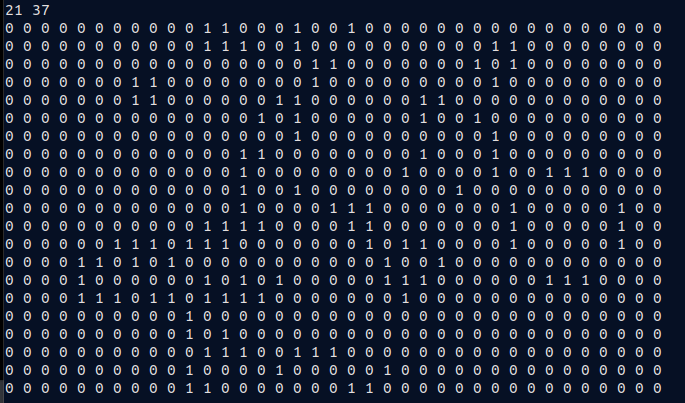
\includegraphics[scale=0.5]{wyjscie}
	\caption{Plik tekstowy z generacj\k{a} wyj\'sciow\k{a}}
        \label{fig:wyjscie}
\end{figure}

\newpage

\part{Implementacja programu}

\section{Informacje og\'olne}

\subsection{Nowy diagram modu\l{}\'ow}
\quad W celu zapewnienia wi\k{e}kszej czytelno\'sci kodu programu oraz dodania nowych funkcjonalno\'sci, 
zosta\l{} ponownie sporz\k{a}dzony diagram modu\l{}\'ow (patrz \textit{Rysunek \ref{fig:Diagram}}).

        \begin{figure}[h]
                \centering
                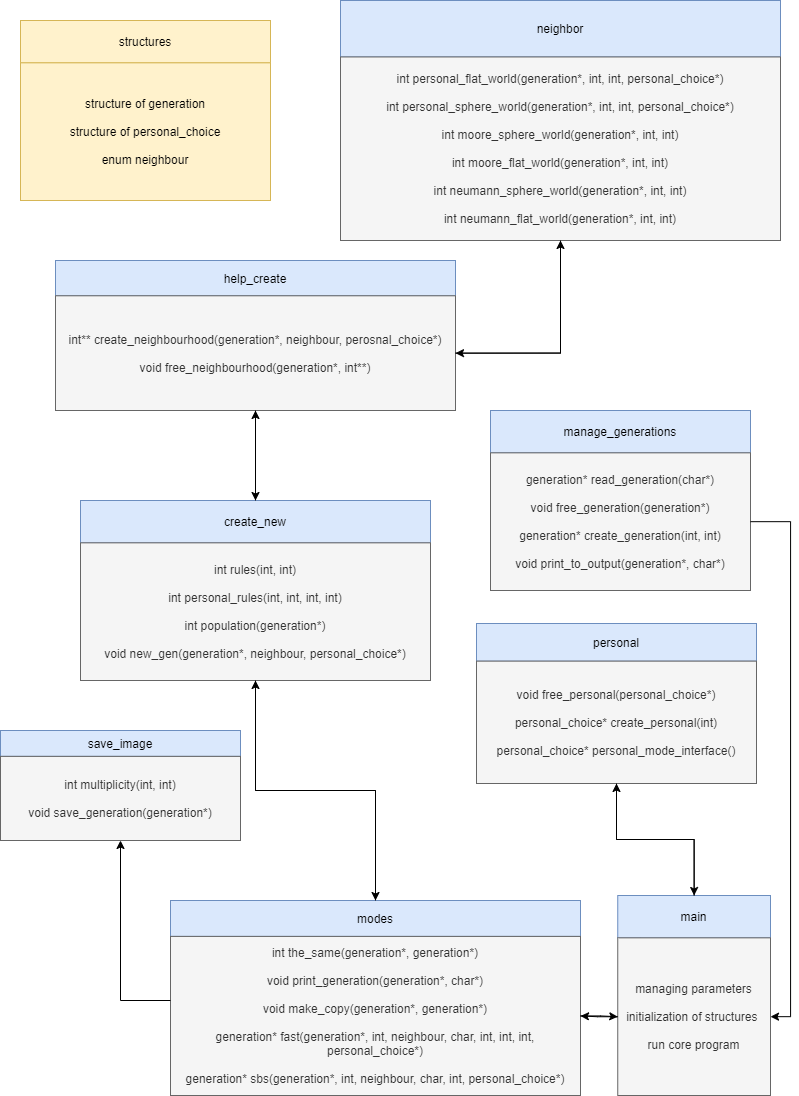
\includegraphics[scale=0.37]{Diagram}
		\caption{Ko\'ncowy diagram modu\l{}\'ow}
		\label{fig:Diagram}
        \end{figure}

\subsection{Informacje og\'olne o zmianach w modu\l{}ach}

\quad Struktury, kt\'ore mia\l{}y by\'c zdefiniowane w module \textbf{main}, 
zosta\l{}y przeniesione do osobnego modu\l{}u pe\l{}ni\k{a}cego rol\k{e} pliku nag\l{}\'owkowego.


Dodatkowo zosta\l{}a dodana nowa struktura \textbf{personal\_choice}, u\.zywana do obs\l{}ugi w\l{}asnego trybu s\k{a}siedztwa.


Podobnie, obs\l{}ug\k{e} plik\'ow przeniesiono do nowego modu\l{}u \\ \textbf{manage\_generations}, natomiast w module \textbf{main} jest ona tylko wywo\l{}ywana.

Zosta\l{} wprowadzony nowy typ s\k{a}siedztwa, a co za tym idzie pojawi\l{} si\k{e} kolejny modu\l{} \textbf{personal}, kt\'ory obs\l{}uguje jego podstawowe funkcje.

Z powodu u\.zywania zmiennych strukturalnych jako argument\'ow wielu funkcji, \textbf{structures} jest wykorzystywane we wszystkich modu\l{}ach.



\section{Informacje szczeg\'o\l{}owe o modu\l{}ach}

\subsection{main}

\quad Modu\l{} zawiera tylko jedn\k{a} funkcj\k{e} \textbf{main}.
Skupia si\k{e} on wy\l{}\k{a}cznie na obs\l{}udze parametr\'ow wsadowych, tworzeniu inicjalizacji g\l{}\'ownych zmiennych oraz uruchamianiu kluczowych funkcji z innych modu\l{}\'ow.
Zawiera wszelkie potrzebne obs\l{}ugi b\l{}\k{e}d\'ow.


Podstawow\k{a} zmian\k{a} wzgl\k{e}dem \textit{"Specyfikacji implementacyjnej automatu kom\'orkowego"} jest przeniesienie obs\l{}ugi plik\'ow oraz definiowanie struktur do osobnych modu\l{}\'ow.

\subsection{personal}

\quad Ca\l{}y modu\l{} jest wzgl\k{e}dnie nowy wobec poprzednich specyfikacji.
Powsta\l{} na potrzeby kontrolowania nowego trybu s\k{a}siedztwa \texttt{PERSONAL}.


Modu\l{} zawiera trzy funkcje (patrz \textit{Tabela \ref{table:Tabela1}}).

\subsection{modes}

\quad Funkcjonowanie tego modu\l{}u nie zmieni\l{}o si\k{e}, jednak parametry funkcji tryb\'ow zosta\l{}y rozszerzone.
Ponadto dodano trzy nowe funkcje wspomagaj\k{a}ce dzia\l{}anie tryb\'ow (patrz \textit{Tabela \ref{table:Tabela2}}).


\subsection{save\_image}

\quad Ze wzgl\k{e}du na \l{}atwiejsz\k{a} implementacj\k{e}, wbrew pierwotnym za\l{}o\.zeniom, 
obraz generacji nie jest zapisywany do pliku o rozszerzeniu \textbf{bmp}, a \textbf{pgm}.
Zosta\l{}a dodana tak\.ze funkcja pomocnicza licz\k{a}ca wielokrotno\'s\'c liczby (patrz \textit{Tabela \ref{table:Tabela3}}).


\subsection{manage\_generations}

\quad Nowopowsta\l{}y modu\l{} w celu odci\k{a}\.zenia \textbf{main}, zawiera podstawowe funkcje obs\l{}uguj\k{a}ce zmienne typu \textbf{\texttt{generation}} (patrz \textit{Tabela \ref{table:Tabela4}}).

\subsection{create\_new}

\quad Modu\l{} zosta\l{} rozszerzony o now\k{a} funkcj\k{e} zasad, dla nowego trybu s\k{a}siedztwa.
Dodano tak\.ze funkcj\k{e} licz\k{a}c\k{a} populacj\k{e} (patrz \textit{Tabela \ref{table:Tabela5}}).


\subsection{help\_create}

\quad Do modu\l{}u dodano jedn\k{a} funkcj\k{e} czyszcz\k{a}c\k{a} dwuwymiarow\k{a} tablic\k{e} s\k{a}siedztwa.
Natomiast funkcja tworz\k{a}ca s\k{a}siedztwo zosta\l{}a wzbogadzona o jeden argument dla spersonalizowanego typu s\k{a}siedztwa (patrz \textit{Tabela \ref{table:Tabela6}}).


\subsection{neighbor}

\quad Opr\'ocz tryb\'ow s\k{a}siedztwa opisanych w specyfikacjach, zosta\l{}y dodane dwa nowe.
By\l{}o to spowodowane dodaniem opcji spersonalizowania regu\l{} s\k{a}siedztwa (patrz \textit{Tabela \ref{table:Tabela7}}).


\subsection{stuctures}
\quad Struktury zosta\l{}y wyodr\k{e}bnione w osobny modul{}.
Dodatkowo utowrzona zosta\l{}a nowa struktura \textbf{personal\_choice}, w celu obs\l{}ugi spersonalizowanego trybu s\k{a}siedztwa.


Nowa struktura zawiera cztery parametry:\\
 - \textbf{dies} typu \textbf{int}, okre\'slaj\k{a}ca od jakiej liczby s\k{a}siad\'ow kom\'orka ma umrze\'c. \\
 - \textbf{comes\_back} typu \textbf{int}, okre\'slaj\k{a}ca od jakiej liczby s\k{a}siad\'ow kom\'orka ma o\.zy\'c. \\
 - \textbf{personal\_neighbours} typu \textbf{int}, okre\'slaj\k{a}ca maksymaln\k{a} liczb\k{e} s\k{a}siad\'ow kom\'orki. \\
 - \textbf{neighbours\_index} typu \textbf{int*}, zapami\k{e}tuj\k{a}ca indeksy s\k{a}siad\'ow kom\'orki. \\

\section{Dodatkowe implementacje}

\subsection{Makefile}

\quad Opr\'ocz podstawowych funkcji zosta\l{} utworzony \textbf{Makefile} w celu \l{}atwiejszego uruchamiania programu.


Zawieraj\k{a} si\k{e} w nim wszelkie mo\.zliwe rodzaje kompilacji oraz uruchomienia.
Przy zmianie tylko argument\'ow wej\'sciowych uruchomienia programu, mo\.zna wymienia\'c rodzaje kompilacji.
Po ka\.zdym uruchomieniu nast\k{e}puje usuni\k{e}cie pliku wynikowego.


Przyk\l{}ad podstawowego pliku wynikowego:\\ \\
\textbf{\texttt{game: \\
\$(CC) -g Moduly/main.c Moduly/modes.c Moduly/save\_image.c \\
Moduly/manage\_generations.c Moduly/create\_new.c \\ 
Moduly/help\_create.c Moduly/neighbor.c Moduly/personal.c\\
-Wall -pedantic -o game\\
}}
\\
\\

Przyk\l{}ad implementacji uruchomienia w trybie sbs:\\ \\
\textbf{\texttt{run\_sbs: game \\
        ./change --in plikin.txt --out plikout.txt  -n 20 --how Ps -m sbs\\ 
        rm -f change\\
}}

Dodatkowo zosta\l{}y zaimplementowane opcje wyczyszczenia zawarto\'sci katalog\'ow \textbf{\texttt{'"Generacje\_Wyjsciowe"'}} oraz \textbf{\texttt{'"Obrazy"'}}:\\ \\
\textbf{\texttt{remove\_out:\\
        rm Generacje\_Wyjsciowe/*.txt \\
remove\_image:\\
        rm Obrazy/generation*\\
}}


Ponadto w fazie testowania zosta\l{}y napisane formu\l{}y uruchomienia poszczeg\'olnych tes\'ow, w celu sprawdzenia poprawno\'sci otrzymywanych wynik\'ow.

\subsection{Makra}

\quad W celu zwi\k{e}kszenia mo\.zliwo\'sci personalizacji wynik\'ow programu, napisane zosta\l{}y zmienne w postaci makr.
Dotycz\k{a} one takich element\'ow jak \'scie\.zki do plik\'ow z generacjami wej\'sciowymi i wyj\'sciowymi, 
rozmiar boku kom\'orki przy zapisie obrazu oraz szybko\'s\'c wy\'swietlania generacji podczas uruchomienia trybu \texttt{FAST}.

\section{Podsumowanie zmian}

\quad Do ka\.zdego modu\l{}u zosta\l{}y wprowadzone zmiany. Niekt\'ore powsta\l{}y od nowa (\textbf{manage\_generations}, \textbf{structures}, \textbf{personal}), 
a zdecydowana wi\k{e}kszo\'s\'c zosta\l{}a rozszerzona o dodatkowe funkcje.
Zosta\l{} tak\.ze dodany \textbf{Makefile} w celu u\l{}atwienia uruchamiania.
Ponadto, w celu mo\.zliwo\'sci personalizacji dzia\l{}ania programu, zosta\l{} dodany nowy tryb s\k{a}siedztwa \texttt{PERSONAL} oraz makra,
kt\'ore przy kompilacji programu pozwalaj\k{a} nam zmieni\'c niekt\'ore parametry.
Ze wzgl\k{e}du na u\l{}atwienia implementacyjne zapis generacji odbywa si\k{e} do pliku graficznego o rozszerzeniu \textbf{pgm}.

\newpage
\section{Tabele}

\begin{table}[h!]
	\centering
	
	\caption{Tablica funkcji modu\l{}u \textbf{personal}}
        \label{table:Tabela1}

	\begin{tabular}{| c | c | c | p{3cm} |}

                \hline
                typ funkcji & nazwa funkcji & argumenty funkcji & cel funkcji \\ \hline \hline

                void    & free\_personal  & personal\_choice* & zwolnienie pami\k{e}ci zmiennej typu \textbf{personal} \\ \hline

                personal\_choice* & create\_personal & int & inicjalizacja zmiennej typu \textbf{personal} \\ \hline

                perosnal\_choice* & personal\_mode\_interface &  & przypisanie warto\'sci zmiennej typu \textbf{personal} zgodnie z danymi pobranymi od u\.zytkownika \\ \hline

        \end{tabular}
\end{table}

\begin{table}[h!]
	\centering

	\caption{\label{table:Tabela2}Tablica funkcji modu\l{}u \textbf{modes}}

        \begin{tabular}{| c | c | c | p{3cm}  |}
                \hline
                typ funkcji & nazwa funkcji & argumenty funkcji & cel funkcji \\ \hline \hline

                void & print\_generation & generation* & wy\'swietlenie pojedy\'nczej \\
                & & char* & generacji na ekran \\ \hline

                int & the\_same & generation* & sprawdzenie czy dwie generacje  \\
                & & generation* & wygl\k{a}daj\k{a} tak samo\\ \hline

                void & make\_copy & generation* & zapisanie generacji\\
                & & generation* & jednej zmiennej do drugiej \\ \hline

                generation* & fast & generation* & uruchomienie \\
                & & int & trybu\\
                & & neighbour & fast \\
                & & char & \\
                & & int & \\
                & & int & \\
                & & int & \\
                & & personal\_choice* & \\ \hline

                generation* & sbs & generation* & uruchomienie \\
                & & int & trybu\\
                & & neighbour & sbs \\
                & & char & \\
                & & int & \\
                & & personal\_choice* & \\ \hline
        \end{tabular}
\end{table}

\newpage

\begin{table}[h!]
	\centering

	\caption{\label{table:Tabela3} Tablica funkcji modu\l{}u \textbf{save\_image}}
        
	\begin{tabular}{| c | c | c | p{3cm}  |}
                \hline
                typ funkcji & nazwa funkcji & argumenty funkcji & cel funkcji \\ \hline \hline

                int & mupltiplicity & int & liczenie jaka to \\
                & & int & wielokrotno\'s\'c danej liczby\\ \hline

                void & save\_generation & generation* & zapisanie generacji do pliku graficznego o rozszerzeniu \textbf{pgm} \\ \hline

        \end{tabular}
\end{table}




\begin{table}[h!]
	\centering
	\caption{\label{table:Tabela4}Tablica funkcji modu\l{}u \textbf{manage\_generations}}
        \begin{tabular}{| c | c | c | p{3cm}  |}
                \hline
                typ funkcji & nazwa funkcji & argumenty funkcji & cel funkcji \\ \hline \hline

                generation* & read\_generation & char* & przypisanie warto\'sci zmiennej typu \textbf{generation} zgodnie z danymi z pliku     \\ \hline
                void & free\_generation & generation* & zwolnienie pami\k{e}ci przypisanej dla zmiennej typu \textbf{generation} \\ \hline
                generation* & create\_generation & int & inicjalizacja zmiennej \\
                & & int & typu \textbf{generation}\\ \hline

                void & print\_to\_output & generation* & zapisanie tablicy ostatniej \\
                & & char* & generacji do pliku tekstowego\\ \hline

        \end{tabular}
\end{table}

\newpage


\begin{table}[h!]
	\centering
	\caption{\label{table:Tabela5}Tablica funkcji modu\l{}u \textbf{create\_new}}
        \begin{tabular}{| c | c | c | p{3cm}  |}
                \hline
                typ funkcji & nazwa funkcji & argumenty funkcji & cel funkcji \\ \hline \hline

                int & rules & int & okre\'slenie stanu kom\'orki dla \\
                & & int & nowej generacji w podstawowym uruchomieniu\\ \hline

                int & personal\_rules & int & okre\'slenie stanu \\
                & & int & kom\'orki dla nowej\\
                & & int & generacji w \\
                & & int & spersonalizowanym uruchomieniu\\ \hline

                int & population & generation* & zliczenie populacji dla pojedy\'nczej generacji \\ \hline

                void & new\_gen & generation* & utworzenie \\
                & & neighbour & nowej\\
                & & personal\_choice* & generacji\\ \hline


        \end{tabular}
\end{table}




\begin{table}[h!]
	\centering
	\caption{\label{table:Tabela6}Tablica funkcji modu\l{}u \textbf{help\_create}}
        \begin{tabular}{| c | c | c | p{3cm}  |}
                \hline
                typ funkcji & nazwa funkcji & argumenty funkcji & cel funkcji \\ \hline \hline

                int** & create\_neighbourhood & generation* & tworzenie \\
                & & neighbour & tablicy \\
                & & personal\_choice* & s\k{a}siedztwa \\ \hline

                void & free\_neighbourhood & generation* & zwolnienie pami\k{e}ci zarezerwowanej \\
                & & int** & dla tablicy s\k{a}siedztwa \\ \hline

        \end{tabular}
\end{table}

\newpage


\begin{table}[h!]
	\centering
	\caption{\label{table:Tabela7}Tablica funkcji modu\l{}u \textbf{neighbor}}
        \begin{tabular}{| c | c | c | p{3cm}  |}
                \hline
                typ funkcji & nazwa funkcji & argumenty funkcji & cel funkcji \\ \hline \hline

                int & personal\_flat\_world & int & liczenie s\k{a}siad\'ow \\
                & & int & kom\'orki dla spersonalizowanego \\
                & & int & trybu s\k{a}siedztwa \\
                & & personal\_choice* & w p\l{}askim \'swiecie \\ \hline

                int & personal\_sphere\_world & int & liczenie s\k{a}siad\'ow \\
                & & int & kom\'orki dla spersonalizowanego \\
                & & int & trybu s\k{a}siedztwa \\
                & & personal\_choice* & w sferycznym \'swiecie \\ \hline

                int & moore\_sphere\_world & generation* & liczenie s\k{a}siad\'ow \\
                & & int & kom\'orki dla podstawowego \\
                & & int & trybu s\k{a}siedztwa Moore'a w sferycznym \'swiecie \\ \hline

                int & moore\_flat\_world & generation* & liczenie s\k{a}siad\'ow \\
                & & int & kom\'orki dla podstawowego \\
                & & int & trybu s\k{a}siedztwa Moore'a w p\l{}askim \'swiecie \\ \hline

                int & neumann\_sphere\_world & generation* & liczenie s\k{a}siad\'ow \\
                & & int & kom\'orki dla podstawowego \\
                & & int & trybu s\k{a}siedztwa Neumanna w sferycznym \'swiecie \\ \hline

                int & neumann\_flat\_world & generation* & liczenie s\k{a}siad\'ow \\
                & & int & kom\'orki dla podstawowego \\
                & & int & trybu s\k{a}siedztwa Neumanna w p\l{}askim \'swiecie \\ \hline

        \end{tabular}
\end{table}

\newpage

\part{Sprawozdanie Test\'ow}

\section{Cel test\'ow}

\quad W fazie testowania szczeg\'olna uwaga zosta\l{}a po\'swi\k{e}cona obs\l{}udze b\l{}\k{e}d\'ow pami\k{e}ci, parametr\'ow wej\'sciowych 
oraz zmiennych otrzymanych od u\.zytkownika poprzez interface trybu \texttt{PERSONAL}.
Celem by\l{}o udoskonalenie programu oraz sprawienie by by\l{} mo\.zliwie najlepiej przystosowany do potrzeb u\.zytkownika.

\section{Plan test\'ow}

\quad Opr\'ocz wcze\'sniej zadeklarowanych test\'ow (patrz \textit{"Specyfikacja implementacyjna automatu kom\'orkowego"}) nale\.za\l{}o doda\'c testy dodatkowe.
By\l{}o to spowodowane zmianami i rozszerzeniami w modu\l{}ach programu.


Do dodatkowych test\'ow zaliczaj\k{a} si\k{e}:
\begin{itemize}
	\item sprawdzenie poprawno\'sci obs\l{}ugi parametr\'ow uruchomienia interface'u,
	\item zapis obraz\'ow mimo zako\'nczenia wy\'swietlania nowych generacji, w skutek sytuacji, gdy kolejne generacje s\k{a} identyczne,
	\item obs\l{}uga wprowadzenia zbyt du\.zej liczby znak\'ow dla trybu \texttt{SBS}.
\end{itemize}

\section{Wyniki}

\quad Zgodnie z przewidywaniami, testy wypad\l{}y pomy\'slnie.
W momentach implementacji wyst\k{e}powa\l{}y  b\l{}\k{e}dy, kt\'ore w miare szybko zostawa\l{}y rozwi\k{a}zywane.
Tak\.ze w czasie test\'ow ostatecznych, wszelkie wyniki by\l{}y przewidywalne i prawid\l{}owe.

Sprawdzenie stanu pami\k{e}ci po uruchomieniu programu (patrz \textit{Rysunek \ref{fig:test}}).
\begin{figure}[h!]
        \centering
        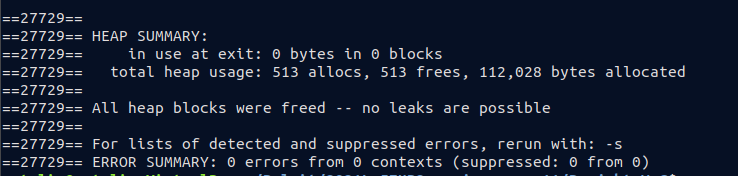
\includegraphics[scale=0.41]{test}
	\caption{Wynik dzia\l{}ania programu \textbf{Valgrind}}
        \label{fig:test}
\end{figure}

\newpage

Sprawdzenie obs\l{}ugi b\l{}\k{e}d\'ow parametr\'ow wej\'sciowych (patrz \textit{Rysunek \ref{fig:test2}}).
\begin{figure}[h!]
        \centering
        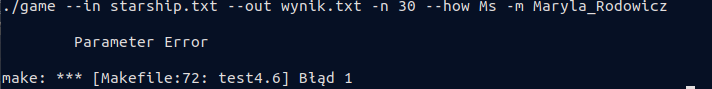
\includegraphics[scale=0.45]{TheOneMarylaunknown}
	\caption{Podanie nieistniej\k{a}cej warto\'sci parametru}
        \label{fig:test2}
\end{figure}

Sprawdzenie obs\l{}ugi b\l{}\k{e}d\'ow dotycz\k{a}cych plik\'ow wej\'sciowych (patrz \textit{Rysunek \ref{fig:test3}}).
\begin{figure}[h!]
        \centering
        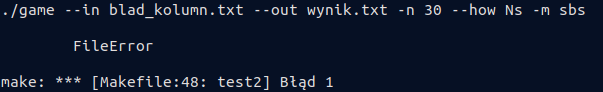
\includegraphics[scale=0.68]{unknown}
	\caption{Pr\'oba u\.zycia niew\l{}a\'sciwego pliku wej\'sciowego}
        \label{fig:test3}
\end{figure}

Podczas korzystania z trybu s\k{a}siedztwa \texttt{PERSONAL}, istnieje mo\.zliwo\'s\'c wprowadzenia b\l{}ednych danych.


Jednym z nich jest powt\'orzenie numeru indeksu.
W tym momencie program przypomni u\.zytkownikowi, \.ze taki indeks ju\.z si\k{e} pojawi\l{} i nale\.zy wybra\'c inny (patrz \textit{Rysunek \ref{fig:test4}}).
\begin{figure}[h!]
        \centering
        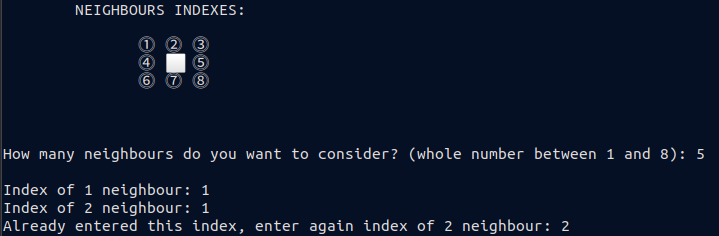
\includegraphics[scale=0.4]{powtorz}
        \caption{Ponowny wyb\'or tego samego indeksu}
        \label{fig:test4}
\end{figure}

Podobnie, u\.zytkownik mo\.ze poda\'c liczb\k{e} wykraczaj\k{a}c\k{a} poza dany przedzia\l{}.
Zostanie on w\'owczas o tym poinformowany, a program zako\'nczy prac\k{e} (patrz \textit{Rysunek \ref{fig:test5}}).
\begin{figure}[h!]
        \centering
	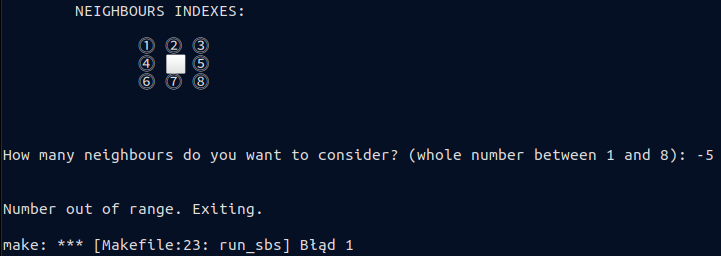
\includegraphics[scale=0.53]{test2}
	\caption{Niepoprawne dane wykraczaj\k{a}ce poza akceptowany przedzia\l{}}
        \label{fig:test5}
\end{figure}

Natomiast, gdy u\.zytkownik poda liter\k{e} zamiast liczby, program zako\'nczy prac\k{e} bez ostrze\.zenia (patrz \textit{Rysunek \ref{fig:test6}}).
\begin{figure}[h!]
        \centering
        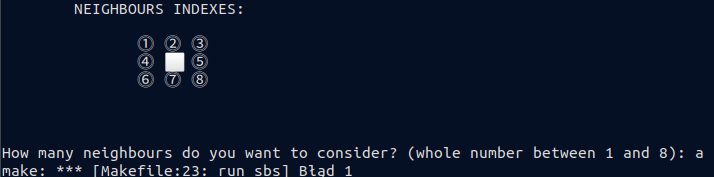
\includegraphics[scale=0.58]{letter}
        \caption{Wprowadzenie zmiennej o niepoprawnym typie}
        \label{fig:test6}
\end{figure}


\section{Zmiany spowodowane wynikami test\'ow}

\quad W czasie tworzenia programu wyst\k{a}pi\l{} tylko jeden moment, w kt\'orym trzeba by\l{}o zmieni\'c jego dzia\l{}anie, aby naprawi\'c b\l{}\k{a}d.
Mia\l{} on miejsce w czasie pobierania argumentu w trybie \texttt{SBS}.
Nale\.za\l{}o pobiera\'c wszelkie dodatkowe znaki, aby nie pozostawa\l{}y w buforze wej\'scia.
W taki spos\'ob ostateczny program przyjmuje tylko ostatni znak przed \textit{\textbf{ENTER}} lub znak \textit{\textbf{e}}, 
je\'sli wyst\k{a}pi\l{} w trakcie wpisywania.

\section{Wnioski na podstawie test\'ow}

\quad Testy wypad\l{}y pomy\'slnie, jednak nie oznacza to, \.ze programu nie mo\.zna bardziej udoskonali\'c.
Program dzia\l{}a zgodnie z pocz\k{a}tkowymi za\l{}o\.zeniami, a wszelkie podstawowe b\l{}\k{e}dy s\k{a} obs\l{}ugiwane.

\newpage

\part{Spostrze\.zenia i uwagi ko\'ncowe}

\section{Osi\k{a}gni\k{e}cie celu projektu}
\quad Program dzia\l{}a prawid\l{}owo, uda\l{}o si\k{e} tak\.ze poprawnie zaimplementowa\'c wszystkie rozszerzenia. 
Mo\.zna zatem uzna\'c, \.ze cel projektu zosta\l{} osi\k{a}gni\k{e}ty.

\section{Elementy niedoskona\l{}e i mo\.zliwe b\l{}\k{e}dy}
\quad Pomimo dobrych funkcjonalno\'sci oraz pomy\'slnie przeprowadzonych test\'ow, program nie zosta\l{} maksymalnie zabezpieczony.
W przypadku zmiany nazw katalog\'ow, program nie zabezpiecza b\l{}\k{e}d\'ow. 
Informuje o naruszeniu pami\k{e}ci, co skutkuje nag\l{}ym zako\'nczeniem jego pracy. 


Podobnie, komunikaty o b\l{}\k{e}dach nie s\k{a} sprecyzowane, co mo\.ze utrudni\'c u\.zytkownikowi zrozumienie niepowodzenia. 


Odczuwalnym ograniczeniem jest brak mo\.zliwo\'sci szybszego zako\'nczenia pracy programu, bez konieczno\'sci przerwania wykonywania pracy Makefile'a.

\section{Ograniczenia programu}
\quad Program ma pewne ograniczenia, wynikaj\k{a}ce z mo\.zliwo\'sci u\.zytego sprz\k{e}tu. 
Je\'sli urz\k{a}dzenie ma ma\l{}o dost\k{e}pnej pami\k{e}ci, poprawne dzia\l{}anie programu mo\.ze by\'c utrudnione a nawet niemo\.zliwe.


Ponadto, zapis obraz\'ow mo\.zliwy jest tylko do pliku o rozszerzeniu bitowym \textbf{pgm}, kt\'orego podgl\k{a}d mo\.ze by\'c utrudniony, 
ze wzgl\k{e}du na mo\.zliwo\'s\'c konieczno\'sci instalowania dodatkowych narz\k{e}dzi.


Uwzgl\k{e}dnione zosta\l{}y tak\.ze nast\k{e}puj\k{a}ce restrykcje dotycz\k{a}ce rozmiaru generacji:
\begin{itemize}
	\item maksymalna liczba kolumn wynosi 50, a wierszy 40 (przez ograniczone wymiary okna konsoli) 
	\item minimalna liczba kolumn i wierszy wynosi 4 (ze wzg\l{}\k{e}du na logik\k{e} zagadnienia)
\end{itemize}

\section{Podsumowanie wsp\'o\l{}pracy}
\quad Wsp\'o\l{}praca przebieg\l{}a bez komplikacji. 
Obie strony by\l{}y bardzo zaanga\.zowane, mo\.zna by\l{}o zauwa\.zy\'c du\.z\k{a} ch\k{e}\'c udoskonalenia projektu.


\end{document}
